\section{CD-Inhalt}
\label{secCDInhalt}
Auf der beiliegenden CD befinden sich folgende \textit{Dateien} und \textbf{Ordner}:
\begin{itemize}
	\item \textbf{Beleg}
	\begin{itemize}
		\item \textit{Beleg.pdf} - dieses Dokument im PDF-Format
		\item \textbf{src} - enth�lt alle LaTeX-Quelldateien f�r die Erstellung des Belegs
		\begin{itemize}
			\item \textbf{img} - enth�lt alle im Beleg eingebundenen Grafiken
		\end{itemize}
	\end{itemize}
\end{itemize}

\section{Usecases}
\label{JumpUseCases}

\begin{table}
	\begin{center}
			\begin{tabular}{|p{3.5cm}|p{9cm}|}
				\hline
				\textbf{Name} & Nutzer anlegen \\
				\hline
				\textbf{Umfang} & Nutzer \\
				\hline
				\textbf{Ebene} & Startseite \\
				\hline
				\textbf{Prim�r-Actor} & Nutzer \\
				\hline
				\textbf{Stakeholder und Interessen} & Nutzer: m�chte sich anmelden/registrieren \\
				\hline
				\textbf{Vorbedingungen} & Nutzer besitzt kein Konto \\
				\hline
				\textbf{Nachbedingungen} & Nutzer besitzt ein Konto \\
				\hline
				\textbf{Standard-Szenario} & \begin{enumerate} \item Nutzer geht auf 'Neuen Benutzer anlegen' \item Nutzer tr�gt Benutzernamen und E-Mail Adresse ein \end{enumerate} \\
				\hline
				\textbf{Erweiterungen} & \begin{enumerate} \item[2a] Benutzername existiert schon. \end{enumerate} \textit{Wiederhole 2. bis erfolgreiche Anmeldung.} \\
				\hline
				\textbf{Spezielle Anforderungen} & Passwort wird generiert und per E-Mail zugesendet. \\
				\hline
			\end{tabular}
		\caption{Usecase : Nutzer anlegen}
		\label{JumpUsecaseNutzeranlegen}
	\end{center}
\end{table}

\begin{table}
	\begin{center}
			\begin{tabular}{|p{3.5cm}|p{9cm}|}
				\hline
				\textbf{Name} & Nutzer-Login \\
				\hline
				\textbf{Umfang} & Nutzer \\
				\hline
				\textbf{Ebene} & Startseite \\
				\hline
				\textbf{Prim�r-Actor} & Nutzer \\
				\hline
				\textbf{Stakeholder und Interessen} & Nutzer: m�chte sich einloggen \\
				\hline
				\textbf{Vorbedingungen} & Nutzer besitzt ein Konto \\
				\hline
				\textbf{Nachbedingungen} & Nutzer ist angemeldet \\
				\hline
				\textbf{Standard-Szenario} & \begin{enumerate} \item Nutzer tr�gt Daten in Login-Felder ein. \item Nutzer klickt auf OK. \item Nutzerspezifische Optionen werden angezeigt. \end{enumerate} \\
				\hline
				\textbf{Erweiterungen} & \begin{enumerate} \item[2a] Login-Daten sind falsch eingegeben. \end{enumerate} \textit{Wiederhole 1. - 2. bis erfolgreicher Login.} \\
				\hline
				\textbf{Spezielle Anforderungen} & Passwort wird verschl�sselt �bertragen \\
				\hline
			\end{tabular}
		\caption{Usecase : Nutzerlogin}
		\label{JumpUsecaseNutzerlogin}
	\end{center}
\end{table}

\begin{table}
	\begin{center}
			\begin{tabular}{|p{3.5cm}|p{9cm}|}
				\hline
				\textbf{Name} & Nutzer l�schen \\
				\hline
				\textbf{Umfang} & Nutzer \\
				\hline
				\textbf{Ebene} & Admin-Page \\
				\hline
				\textbf{Prim�r-Actor} & Admin \\
				\hline
				\textbf{Stakeholder und Interessen} & \begin{itemize} \item Admin: m�chte/soll Nutzer aus System entfernen \item Nutzer: m�chte/soll entfernt werden \end{itemize} \\
				\hline
				\textbf{Vorbedingungen} & \begin{itemize} \item Nutzer besitzt ein Konto \item Admin ist angemeldet \end{itemize} \\
				\hline
				\textbf{Nachbedingungen} & Nutzerkonto ist gel�scht \\
				\hline
				\textbf{Standard-Szenario} & \begin{enumerate} \item Admin ruft Nutzeradministration auf. \item Admin w�hlt f�r den Nutzer die Option L�schen. \item Nutzer wird nicht mehr in Liste angezeigt. \end{enumerate} \\
				\hline
				\textbf{Erweiterungen} & keine \\
				\hline
			\end{tabular}
		\caption{Usecase : Nutzer l�schen}
		\label{JumpUsecaseNutzerLoeschen}
	\end{center}
\end{table}

\begin{table}
	\begin{center}
			\begin{tabular}{|p{3.5cm}|p{9cm}|}
				\hline
				\textbf{Name} & Album anlegen \\
				\hline
				\textbf{Umfang} & Album \\
				\hline
				\textbf{Ebene} & Nutzer-Frontend \\
				\hline
				\textbf{Prim�r-Actor} & Nutzer \\
				\hline
				\textbf{Stakeholder und Interessen} & Nutzer: m�chte ein neues Album anlegen \\
				\hline
				\textbf{Vorbedingungen} & Nutzer ist angemeldet. \\
				\hline
				\textbf{Nachbedingungen} & Ein neues Album wurde angelegt. \\
				\hline
				\textbf{Standard-Szenario} & \begin{enumerate} \item Nutzer klickt auf 'Neues Album'. \item Nutzer tr�gt Albuminformationen ein. \item Nutzer klickt auf OK. \item Das neue Album wird angezeigt. \end{enumerate} \\
				\hline
				\textbf{Erweiterungen} & \begin{enumerate} \item[2a] Nutzer l�dt zus�tzlich Bilder f�r das Album hoch (\nameref{JumpUsecaseBildHochladen}) \item[3a] Ein Album mit demselben Namen existiert bereits. \end{enumerate} \textit{Bei 3a: Wiederhole 2 bis Albumname noch nicht vorhanden.} \\
				\hline
			\end{tabular}
		\caption{Usecase : Album anlegen}
		\label{JumpUsecaseAlbumAnlegen}
	\end{center}
\end{table}

\begin{table}
\begin{center}
			\begin{tabular}{|p{3.5cm}|p{9cm}|}
				\hline
				\textbf{Name} & Album bearbeiten \\
				\hline
				\textbf{Umfang} & Album \\
				\hline
				\textbf{Ebene} & Nutzer-Frontend \\
				\hline
				\textbf{Prim�r-Actor} & Nutzer \\
				\hline
				\textbf{Stakeholder und Interessen} & Nutzer: m�chte Album bearbeiten \\
				\hline
				\textbf{Vorbedingungen} & Nutzer ist angemeldet. \\
				\hline
				\textbf{Nachbedingungen} & Das Album wurde ge�ndert. \\
				\hline
				\textbf{Standard-Szenario} & \begin{enumerate} \item Nutzer klickt auf das Album \item Nutzer klickt auf 'Bearbeiten'. \item Nutzer tr�gt neue Albuminformationen ein. \item Nutzer klickt auf OK. \item Das bearbeitete Album wird angezeigt. \end{enumerate} \\
				\hline
				\textbf{Erweiterungen} & \begin{enumerate} \item[3a] Nutzer l�dt zus�tzlich Bilder f�r das Album hoch. (\nameref{JumpUsecaseBildHochladen}) \item[3b] Nutzer l�scht bereits vorhandene Bilder (\nameref{JumpUsecaseBildLoeschen}) \item[4a] Ein Album mit demselben Namen existiert bereits. \end{enumerate} \textit{Bei 4a: Wiederhole 3 bis Albumname noch nicht vorhanden.} \\
				\hline
			\end{tabular}
		\caption{Usecase : Album bearbeiten}
		\label{JumpUsecaseAlbumBearbeiten}
	\end{center}
\end{table}

\begin{table}
	\begin{center}
			\begin{tabular}{|p{3.5cm}|p{9cm}|}
				\hline
				\textbf{Name} & Bild hochladen \\
				\hline
				\textbf{Umfang} & Album \\
				\hline
				\textbf{Ebene} & Nutzer-Frontend \\
				\hline
				\textbf{Prim�r-Actor} & Nutzer \\
				\hline
				\textbf{Stakeholder und Interessen} & Nutzer: m�chte Bild hochladen \\
				\hline
				\textbf{Vorbedingungen} & Nutzer ist angemeldet. \\
				\hline
				\textbf{Nachbedingungen} & Das Bild wurden hochgeladen. \\
				\hline
				\textbf{Standard-Szenario} & \begin{enumerate} \item Nutzer klickt auf 'Album bearbeiten' des jeweiligen Albums \item Nutzer klickt auf 'Durchsuchen' \item Nutzer w�hlt Bild aus. \item Nutzer klickt auf OK. \item Nutzer klickt auf 'Alle Hochladen'. \item Nutzer klickt auf 'speichern'. \end{enumerate} \\
				\hline
				\textbf{Erweiterungen} &   \\
				\hline
			\end{tabular}
		\caption{Usecase : Bild hochladen}
		\label{JumpUsecaseBildHochladen}
	\end{center}
\end{table}

\begin{table}
	\begin{center}
			\begin{tabular}{|p{3.5cm}|p{9cm}|}
				\hline
				\textbf{Name} & Bild bearbeiten \\
				\hline
				\textbf{Umfang} & Album \\
				\hline
				\textbf{Ebene} & Nutzer-Frontend \\
				\hline
				\textbf{Prim�r-Actor} & Nutzer \\
				\hline
				\textbf{Stakeholder und Interessen} & Nutzer: m�chte Bildinformationen �ndern \\
				\hline
				\textbf{Vorbedingungen} & Nutzer ist angemeldet. \\
				\hline
				\textbf{Nachbedingungen} & Die Bildinformationen wurden ge�ndert. \\
				\hline
				\textbf{Standard-Szenario} & \begin{enumerate} \item Nutzer klickt auf 'Album bearbeiten' des jeweiligen Albums \item Nutzer klickt auf 'bearbeiten' beim jeweiligen Bild \item Nutzer �ndert Bildinformationen. \item Nutzer klickt auf 'speichern'. \item  \end{enumerate} \\
				\hline
				\textbf{Erweiterungen} &   \\
				\hline
			\end{tabular}
		\caption{Usecase : Bild bearbeiten}
		\label{JumpUsecaseBildbearbeiten}
	\end{center}
\end{table}

\begin{table}
	\begin{center}
			\begin{tabular}{|p{3.5cm}|p{9cm}|}
				\hline
				\textbf{Name} & Bild l�schen \\
				\hline
				\textbf{Umfang} & Album \\
				\hline
				\textbf{Ebene} & Nutzer-Frontend \\
				\hline
				\textbf{Prim�r-Actor} & Nutzer \\
				\hline
				\textbf{Stakeholder und Interessen} & Nutzer: m�chte Bild l�schen \\
				\hline
				\textbf{Vorbedingungen} & Nutzer ist angemeldet. \\
				\hline
				\textbf{Nachbedingungen} & Das Bild wurden gel�scht. \\
				\hline
				\textbf{Standard-Szenario} & \begin{enumerate} \item Nutzer klickt bei dem gew�nschten Bild auf 'l�schen' unter Album bearbeiten  \item Nutzer best�tigt Nachfrage mit 'Ja'. \item Nutzer klickt auf 'speichern'. \end{enumerate} \\
				\hline
				\textbf{Erweiterungen} &   \\
				\hline
			\end{tabular}
		\caption{Usecase : Bild l�schen}
		\label{JumpUsecaseBildLoeschen}
	\end{center}
\end{table}

\begin{table}
	\begin{center}
			\begin{tabular}{|p{3.5cm}|p{9cm}|}
				\hline
				\textbf{Name} & Album anzeigen \\
				\hline
				\textbf{Umfang} & Album \\
				\hline
				\textbf{Ebene} & Nutzer-Frontend \\
				\hline
				\textbf{Prim�r-Actor} & Nutzer \\
				\hline
				\textbf{Stakeholder und Interessen} & Nutzer: m�chte Album ansehen \\
				\hline
				\textbf{Vorbedingungen} & Nutzer ist angemeldet. \\
				\hline
				\textbf{Nachbedingungen} & Das Album wird angezeigt. \\
				\hline
				\textbf{Standard-Szenario} & \begin{enumerate} \item Nutzer klickt auf 'Album�bersicht'  \item Nutzer w�hlt Album aus.  \end{enumerate} \\
				\hline
				\textbf{Erweiterungen} &   \\
				\hline
			\end{tabular}
		\caption{Usecase : Album anzeigen}
		\label{JumpUsecaseAlbumanzeigen}
	\end{center}
\end{table}



\newpage
\section{UML-Diagramme}
\label{secAnhang}

\section{Listings}

\subsection{XML-Dokumente}

\begin{lstlisting}[caption=Beispiel f�r einen Eintrag in der nutzers.xhtml,label=JumpListingNutzerXML,language=XML]
<nutzer>
    <id>0</id>
    <name>Karl</name>
    <password>98f6bcd4621d373cade4e832627b4f6</password>
    <email>karl@web.de</email>
</nutzer>
\end{lstlisting}
\begin{lstlisting}[caption=Beispiel f�r einen Eintrag in der alben.xhtml,label=JumpListingAlbumXML,language=XML]
<album>
    <id>0</id>
    <name>G�rlitz</name>
    <password>9e229f114819f62674b5b1a031a9f91</password>
    <description>Bilder �ber die Stadt G�rlitz.</description>
    <nutzer>0</nutzer>
</album>\end{lstlisting}
\begin{lstlisting}[caption=Beispiel f�r einen Eintrag in der bilder.xhtml,label=JumpListingBildXML,language=XML]
<bild>
    <id>2</id>
    <name>Vogtshof Innenhof</name>
    <description>Studenten beim Grillen</description>
    <ispublic>false</ispublic>
    <date>2011-02-21 19:05:01</date>
    <fileposition>/pics/Vogtshof_Innenhof_3.jpg</fileposition>
    <album>0</album>
    <position>
        <latitude>51.148833</latitude>
        <longitude>51.148833</longitude>
        <altitude>123</altitude>
        <direction>120</direction>
    </position>
</bild>
\end{lstlisting}

\subsection{Java-Code}

\begin{lstlisting}[caption=Die Klasse MockAlbumConnector,label=JumpListingMockAlbumConnector]
public class MockAlbumConnector implements IAlbumConnector {
  //Durch Mehrere HashMaps kann schnell und einfach auf bestimmte Alben zugegriffen werden
  private final HashMap<Integer, Document> albenIDMap;
  private final HashMap<String, Document> albenNameMap;
  private final HashMap<Integer, Document> albenNutzerIDMap;
  private final HashMap<String, Document> albenDescriptionMap;
  int id = -1;

  public MockAlbumConnector(){
    this.albenIDMap = new HashMap<Integer,Document>();
    this.albenNameMap = new HashMap<String,Document>();
    this.albenNutzerIDMap = new HashMap<Integer,Document>();
    this.albenDescriptionMap = new HashMap<String,Document>();
    //Passwortverschl�sselung f�r ein Album
    String password = "goerlitz";
    try {
      MessageDigest md = MessageDigest.getInstance("md5");
      byte[] digest = md.digest(password.getBytes());
      StringBuffer hexString = new StringBuffer();
      for (int i = 0; i < digest.length; i++) {
        hexString.append(Integer.toHexString(0xFF & digest[i]));
      }
      password = hexString.toString();
    } catch (NoSuchAlgorithmException e) {
      e.printStackTrace();
    }
    //Erstellen eines neuen Documents f�r ein Album
    this.addAlbum("G�rlitz", password, "Bilder �ber die Stadt G�rlitz.", 0);
    ...
  }
  ...
  public Document getAlbumByID(int id) throws ConnectException, IllegalArgumentException {
    if(this.albenIDMap.containsKey(id))
      return this.albenIDMap.get(id);
    else
      throw new IllegalArgumentException("");
  }
  ...
  public Document getAllAlben() throws ConnectException {
    	...
      DocumentBuilderFactory factory = DocumentBuilderFactory.newInstance();
      Document doc = factory.newDocumentBuilder().newDocument();
      Node albenNode = doc.createElement("alben");
      for(Map.Entry<Integer,Document> entry : this.albenIDMap.entrySet()){
        albenNode.appendChild(doc.adoptNode(entry.getValue().getFirstChild()));
      }
      doc.appendChild(albenNode);
      return doc;
      ...
  }

  //Liefert nur bestimmte Alben
  public Document getAlbenForNutzer(int nutzerID) throws ConnectException, IllegalArgumentException {
    	...
      DocumentBuilderFactory factory = DocumentBuilderFactory.newInstance();
      Document doc = factory.newDocumentBuilder().newDocument();
      Node albenNode = doc.createElement("alben");
      for(Map.Entry<Integer,Document> entry : this.albenIDMap.entrySet()){
        if(entry.getValue().getElementsByTagName("nutzer").item(0).getTextContent().equals(""+nutzerID))
          albenNode.appendChild(doc.adoptNode(entry.getValue().getFirstChild()));
      }
      doc.appendChild(albenNode);
      return doc;
      ...
  }
  ...
}
\end{lstlisting}

\begin{lstlisting}[caption=Erweiterung der Klasse Authenticator,label=JumpListingAuthenticator]
public class ExistAuthentificator extends Authenticator {
    protected PasswordAuthentication getPasswordAuthentication(){
        String promptString = getRequestingPrompt();
        String hostname = getRequestingHost();
        InetAddress ipaddr = getRequestingSite();
        int port = getRequestingPort();
        String username = USERNAME;
        String password = PASSWORD;
        return new PasswordAuthentication(username, password.toCharArray());
    }
}
\end{lstlisting}

\begin{lstlisting}[caption=Umsetzung des Singleton-Patterns f�r die Klasse DBConnector,label=JumpDBZugriffSingleton]
private DBConnector(){
  this.location = "http://193.174.103.76:8088/exist/rest/db/";
}
...
private static DBConnector INSTANCE = new DBConnector();

public static DBConnector getInstance(){
  return DBConnector.INSTANCE;
}
...
public synchronized Document executeGetRequest(...){
...
}
\end{lstlisting}

\begin{lstlisting}[caption=Methode zum Erstellen der Marker, label=lstMakeMarker, language=Java]
    public void makeMarker() {
        simpleModel = new DefaultMapModel();
        AlbumController ac = (AlbumController) GPicSUtil.getBean("albumController");
        bilder = ac.getBilder();
        Polyline polyline = new Polyline();
        for (int i = 0; i < ac.getBilder().size(); i++){
            Bild bild = bilder.get(i);

            LatLng coord = new LatLng(Double.parseDouble(bild.getLatitude()), Double.parseDouble(bild.getLongitude()));

            polyline.getPaths().add(coord);

            Marker m  = new Marker(coord, bild.getName(), bild.getPath());

            simpleModel.addOverlay(m);
        }

        polyline.setStrokeWeight(5);
        polyline.setStrokeColor("#FF9900");
        polyline.setStrokeOpacity(0.7);

        simpleModel.addOverlay(polyline);
    }
\end{lstlisting}

\begin{lstlisting}[caption=Methode zur Erzeugung eines zuf�llligen Passworts, label=lstRandomPasswort, language=Java]
public String erzeugeZufallsPasswort(int length) {
        String allowedChars = "0123456789abcdefghijklmnopqrstuvwxyz";
        Random rand = new Random();
        int max = allowedChars.length();
        StringBuffer buffer = new StringBuffer();
        for (int i = 0; i < length; i++) {
            int value = rand.nextInt(max);
            buffer.append(allowedChars.charAt(value));
        }
        return buffer.toString();
    }
\end{lstlisting}

\begin{lstlisting}[caption=Methode f�r die MD5-Verschl�sselung, label=lstEncryptPasswort, language=Java]
public String encryptWithMD5(String passwort){
        StringBuffer hexString = new StringBuffer();
        try {
            MessageDigest md = MessageDigest.getInstance("md5");
            byte[] digest = md.digest(passwort.getBytes());
            for (int i = 0; i < digest.length; i++) {
                hexString.append(Integer.toHexString(0xFF & digest[i]));
            }
        } catch (NoSuchAlgorithmException e) {
            e.printStackTrace();  //To change body of catch statement use File | Settings | File Templates.
        }
        return hexString.toString();
    }
\end{lstlisting}

\begin{lstlisting}[caption=Methode f�r den Mailversand, label=lstMailversand, language=Java]
public String sendPasswortEmail() {
        try {
            String tempPasswort = new PasswortUtil().erzeugeZufallsPasswort(16);

            Document doc = conn.getNutzerByName(nutzerNamen);
            getNutzerIDAndEmail(doc);

            Properties props = new Properties();
            props.put("mail.smtp.auth", "true");
            props.put("mail.smtp.host", "mail.gmx.de");
            props.put("mail.smtp.socketFactory.port", "465");
            props.put("mail.smtp.socketFactory.class",
                    "javax.net.ssl.SSLSocketFactory");
            props.put("mail.smtp.port", 465);
            props.setProperty("mail.smtp.ssl.trust", "mail.gmx.de");
            Authenticator aut = new Authenticator() {
                @Override
                protected PasswordAuthentication getPasswordAuthentication() {
                    return new PasswordAuthentication("gpics@gmx.de", "gpics4XML");
                }
            };
            Session session = Session.getInstance(props, aut);
            MessagePropertiesBean msgPB = new MessagePropertiesBean();
            Message mail = new MimeMessage(session);
            mail.setFrom(new InternetAddress("gpics@gmx.de"));
            mail.setRecipients(Message.RecipientType.TO,
                    InternetAddress.parse(email));
            mail.setSubject(msgPB.getPropertiesMessage("mailSubject"));
            mail.setText(msgPB.getPropertiesMessage("mailPart1") + tempPasswort +
                    msgPB.getPropertiesMessage("mailPart2"));
            Transport.send(mail);
            System.out.println("Done");
            setPasswort(tempPasswort);
            conn.updateNutzer(nutzerID, nutzerNamen, passwort, email);
        } catch (NullPointerException e) {
            System.err.println(e.getMessage());  //F�ngt NullPointerabException ab, die bei Unit-Tests auftritt, weil dort der FacesContext null ist.
        } catch (Exception e) {
            e.printStackTrace();
            GPicSUtil.createFacesMessageForID("sendPWMask", e.getMessage(), true);
            return "sendPW";
        }
        try {
            MessagePropertiesBean mPB = new MessagePropertiesBean();
            GPicSUtil.createFacesMessageForID("infoMessages", mPB.getPropertiesMessage("sendMailSuccess"), false);
        } catch (NullPointerException e) {
            System.err.println(e.getMessage()); //F�ngt NullPointerabException ab, die bei Unit-Tests auftritt, weil dort der FacesContext null ist.
        }
        return "index";
    }
\end{lstlisting}

\begin{lstlisting}[caption=Methode zur Behandlung des FileUploadEvents, label=lstHandleFileUpload, language=Java]
public void handleFileUpload(FileUploadEvent event) {
        UploadedFile file = event.getFile();

        try {
            UserController uc = (UserController) GPicSUtil.getBean("userController");
            String username = uc.getNutzerNamen();
            FileOutputStream out = null;
            if(!isNewAlbum){
                out = new FileOutputStream(uploadDir + albumName + "_" + username + "_" + file.getFileName());
            }else{
                out = new FileOutputStream(uploadDir + username + "_" + file.getFileName());
            }
//            FileOutputStream
            out.write(file.getContents());
            out.flush();
            out.close();
            if(!isNewAlbum){
                updateBilderListe(uploadDir + albumName + "_" + username + "_" + file.getFileName());
            }else{
                updateBilderListe(uploadDir + username + "_" + file.getFileName());
            }

            if (!isNewAlbum) {
                //TODO aufruf von ladeAlbum probieren
                AlbumControllerDBUtil util = new AlbumControllerDBUtil();
                setBilder(util.ladeBilderAusDB(albumID));
//            FacesContext.getCurrentInstance().getExternalContext().redirect("createAlbum.xhtml");
            }
        } catch (Exception e) {
            e.printStackTrace();  //To change body of catch statement use File | Settings | File Templates.
        }
        GPicSUtil.createFacesMessageForID("uploader", file.getFileName() + " erfolgreich hochgeladen.", false);
    }
\end{lstlisting}

\begin{lstlisting}[caption=Parameter�bergabe von einer Webseite an den Controller, label=lstFParam, language=XML]
<p:dataGrid id="cgrid" var="b" value="#{createEditAlbumController.bilder}" columns="3" rows="12" paginator="false" effect="true" paginatorTemplate="{CurrentPageReport} {FirstPageLink} {PreviousPageLink} {PageLinks} {NextPageLink} {LastPageLink} {RowsPerPageDropdown}" rowsPerPageTemplate="9,12,15">
....
                            <p:graphicImage value="#{createEditAlbumController.image}" width="20%"
                                            height="20%">
                                <f:param name="name" value="#{b.name}"/>
                            </p:graphicImage>
....
            </p:dataGrid>
\end{lstlisting}

\begin{lstlisting}[caption=Methode zum Laden der Bilder, label=lstGetImage, language=Java]
public StreamedContent getImage() {
        StreamedContent defaultImage = null;
        try {
            defaultImage = GPicSUtil.getStreamContent(uploadDir + "/gpics.jpg");
            String name = FacesContext.getCurrentInstance()
                    .getExternalContext().getRequestParameterMap().get("name");
            if (name != null && !bilder.isEmpty()) {
                StreamedContent content = null;
                for (Bild b : bilder) {
                    if (b.getName().equals(name)) {
                        content = b.getContent();
                    }
                }
                return content;
            }
        } catch (IOException e) {
            e.printStackTrace();  //To change body of catch statement use File | Settings | File Templates.
        }
        return defaultImage;
    }
\end{lstlisting}

\begin{lstlisting}[caption=Methode um Bean aus FacesContext zu holen, label=lstBeanzugriff, language=Java]
public static Object getBean(String beanName){
        FacesContext context = FacesContext.getCurrentInstance();
        Object o =  context.getApplication()
            .getVariableResolver().resolveVariable(context, beanName);
        return o;
    }
\end{lstlisting}

\begin{lstlisting}[caption=Aufruf einer Methode einer anderen Bean, label=lstBeanzugriffAufruf, language=Java]
...
if (dbPasswort.equals(passwort)) {
                eingeloggt = true;
                getNutzerIDAndEmail(doc);
                if (nutzerNamen.equals("Admin")) {
                    admin = true;
                    AdminPageController ac = (AdminPageController) GPicSUtil.getBean("adminPageController");
                    return ac.loadPage();
                }
                OwnAlbumsController oac = (OwnAlbumsController) GPicSUtil.getBean("ownAlbumsController");
                return oac.initAllAlbums();
            }
...
\end{lstlisting}

\subsection{Antwort von Webservice}
\begin{lstlisting}[caption=Antwort einer GoogleMaps Anfrage, label=lstGoogelMaps, language=XML]
<kml xmlns="http://earth.google.com/kml/2.0"><Response>
  <name>goerlitz, Obermarkt, 17</name>
  <Status>
    <code>200</code>
    <request>geocode</request>
  </Status>
  <Placemark id="p1">
    <address>Obermarkt 17, 02826 G�rlitz, Deutschland</address>
    <AddressDetails Accuracy="8" xmlns="urn:oasis:names:tc:ciq:xsdschema:xAL:2.0"><Country><CountryNameCode>DE</CountryNameCode><CountryName>Germany</CountryName><AdministrativeArea><AdministrativeAreaName>Saxony</AdministrativeAreaName><SubAdministrativeArea><SubAdministrativeAreaName>G�rlitz</SubAdministrativeAreaName><Locality><LocalityName>G�rlitz</LocalityName><DependentLocality><DependentLocalityName>G�rlitz</DependentLocalityName><Thoroughfare><ThoroughfareName>Obermarkt 17</ThoroughfareName></Thoroughfare><PostalCode><PostalCodeNumber>02826</PostalCodeNumber></PostalCode></DependentLocality></Locality></SubAdministrativeArea></AdministrativeArea></Country></AddressDetails>
    <ExtendedData>
      <LatLonBox north="51.1583676" south="51.1520724" east="14.9892076" west="14.9829124" />
    </ExtendedData>
    <Point><coordinates>14.9860600,51.1552200,0</coordinates></Point>
  </Placemark>
</Response></kml>

\end{lstlisting}
%	\label{pageValidationCall}
%	\includepdf[landscape, turn=true, pages=-, fitpaper=true]{img/Validation_Call.pdf}
	
\section{Bilder}
\begin{figure}[ht]
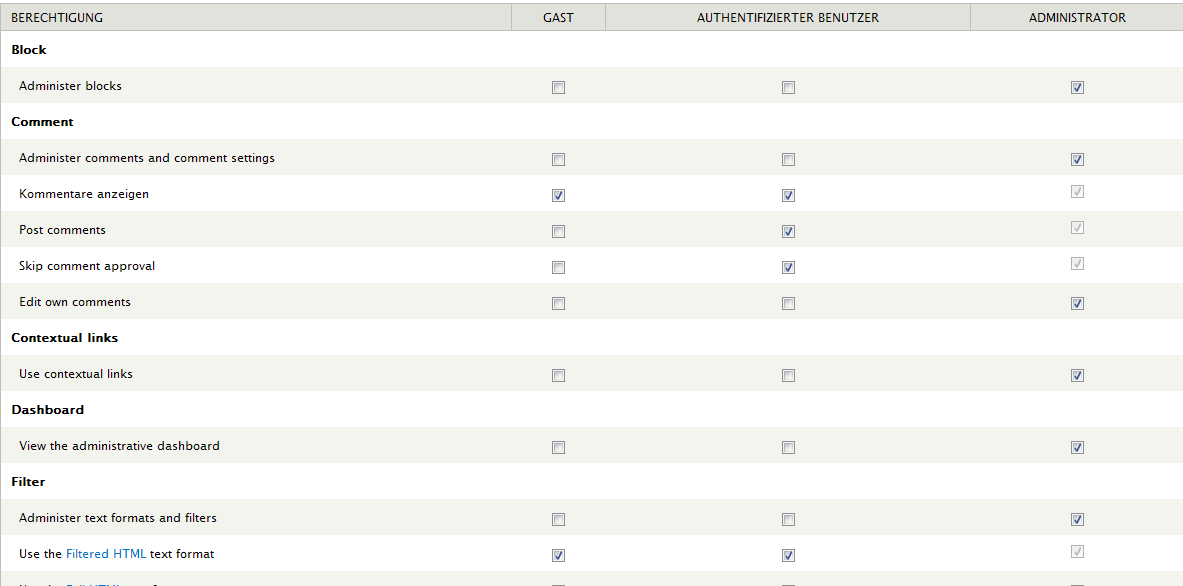
\includegraphics[width=\textwidth]{img/drupal_rollensystem.png}
\caption{Ausschnitt aus rechtebasiertem Rollensystem von Drupal}
\label{fig:drupal_rollen}
\end{figure}
\begin{figure}[ht]
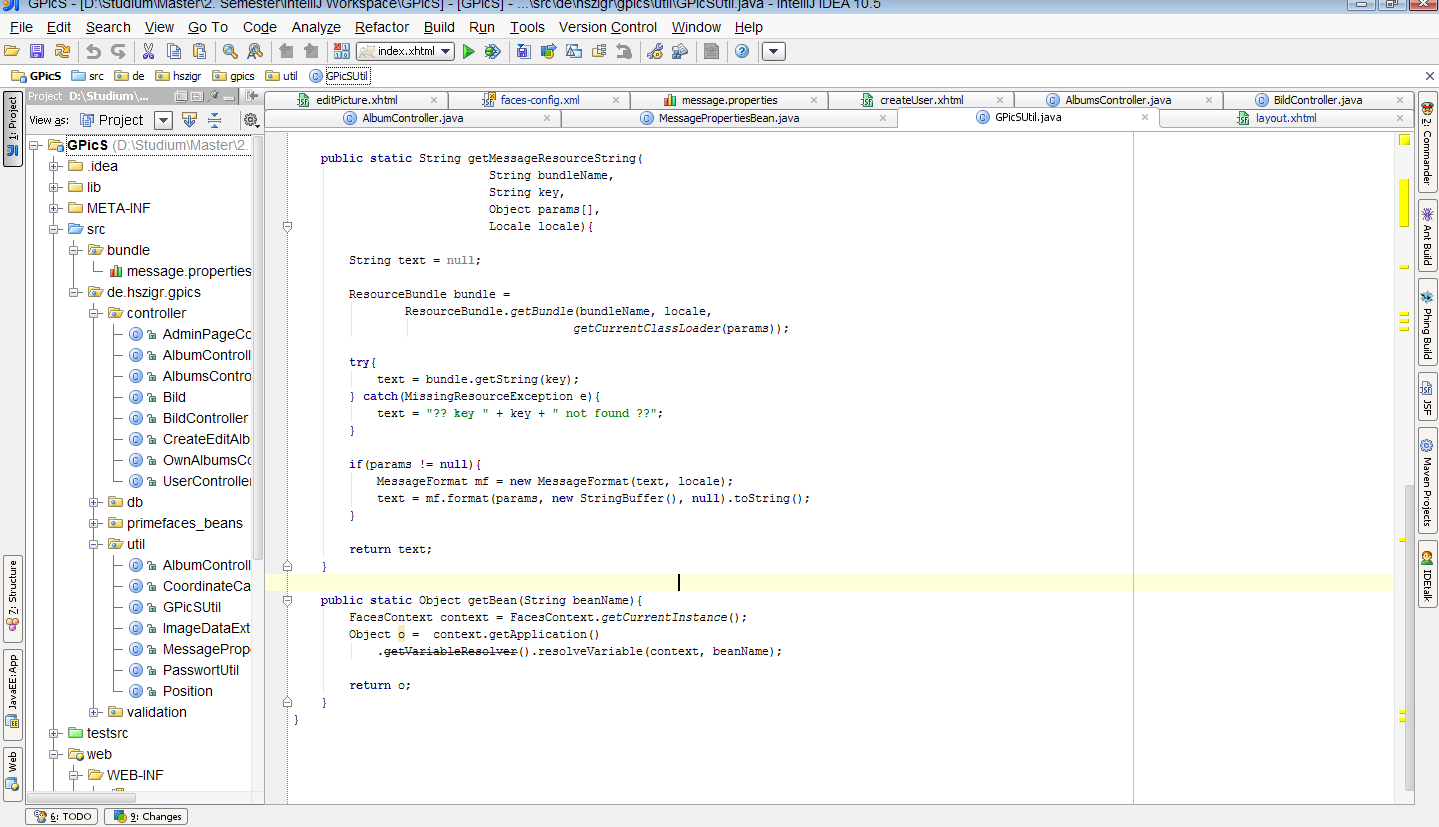
\includegraphics[width=\textwidth]{img/intellij_toolmenu.png}
\caption{Menues rund um den Quellcode}
\label{fig:intellij_menu}
\end{figure}